% ===================== 担当D =====================
\section{担当D — 音響合成（Processing/Minim）}

\subsection{機能一覧}
本担当では，Arduino（担当C）から送信されるシリアル通信データを受信し，
Processing上で音響合成を行い，各楽器音をリアルタイムに出力する機能を実装する．

主な機能は以下の通りである．

\begin{itemize}

  \item シリアル通信受信機能 \\
  Arduinoから送信される4バイトパケット（NOTE\_OFF / NOTE / VEL / LONG）を受信し，
  前音の消音および新規発音イベントとして解釈する．
  ボーレートは115200\,bpsとする．

  \item 受信データパース機能 \\
  受信したバイト列を4バイト単位で解析し，
  NOTE\_OFF（\texttt{1}=前音停止 / \texttt{0}=継続），
  音名インデックス，ベロシティ，および音長（LONG）情報を抽出する．
  LONGは音価（\texttt{2}=2分音符 / \texttt{4}=4分音符 / \texttt{8}=8分音符）を表し，
  発音時にADSRの減衰（Decay）・余韻（Release）時間へ倍率として反映することで
  響き・余韻の長さを調整する（2分音符は長め，4分音符は標準，8分音符は短め）．
  なお，発音中の音を実際に停止するタイミングはLONGではなくNOTE\_OFF=1の受信で制御する．

  \item 音高変換機能 \\
  音名インデックス（C4=0, D4=1, E4=2, F4=3, G4=4, A4=5，休符=6）を
  MIDIノート番号へ変換し，
  $f = 440 \times 2^{(n-69)/12}$\,[Hz] により周波数を算出する．
  変換テーブルは担当Cと合意のうえ実装する．

  \item 音響合成機能 \\
  Minimライブラリを用い，Oscil・ADSR・フィルタ・BitCrusherを
  直列接続したUGenチェーンにより各楽器音をリアルタイムに生成する．

  \item 楽器音色生成機能 \\
  ハイハット・シンバル，バスドラム・スネア，鉄琴，ピアノ，トランペットの
  5パートそれぞれに対し，倍音比率・ADSRパラメータ・フィルタ設定を
  個別に定義し，識別可能な音色を実現する．

  \item 発音・消音制御機能 \\
  NOTE\_OFFフラグ=1のパケット受信時に前音のADSRリリースを開始し，
  続くNOTEバイトが休符（6）でなければ新規発音のアタックを開始する．
  新規発音時はLONG（音価）に応じてADSRの減衰・リリース時間に倍率を乗じ，
  響きの長さを音価に合わせて変化させる（消音の判断自体はLONGでは行わず，
  常にNOTE\_OFF=1の受信で制御する）．
  フェルマータ中は担当Cが次パケットの送信を保留するため，
  Processing側は特別な処理を行わずSustain状態を維持する．
  腕再開後に担当Cから次パケット（NOTE\_OFF=1）が送信された時点で
  リリースを開始し，新たな音の発音へ移行する．

  \item 多重発音機能 \\
  テンポ変化時などNOTE\_OFF=0のパケットを受信した場合，
  前音を強制消音せずに重ねて発音することで，
  音の途切れによる不自然さを回避する．

  \item 操作インターフェース機能 \\
  ハッカソン本番での迅速なセットアップを支援するため，
  シリアルポートの自動接続，マスターボリュームスライダー（0〜100\,\%），
  および受信した4バイトパケット（NOTE\_OFF / NOTE / VEL / LONG）の数値を
  リアルタイム表示するパネルをProcessing上に実装する．

  \item デバッグ・ログ出力機能 \\
  受信パケット（NOTE\_OFF / NOTE / VEL / LONG）のパース結果および発音・消音イベントの
  タイミングをシリアルモニタへ出力し，開発・動作確認を支援する．

\end{itemize}

\subsection{システム構成図}
本構成図では，担当D（Processing/Minim）の内部構成と，
上流の担当C（Arduino子機）および下流のスピーカー出力との接続関係を示す．

\begin{figure}[H]
    \centering
    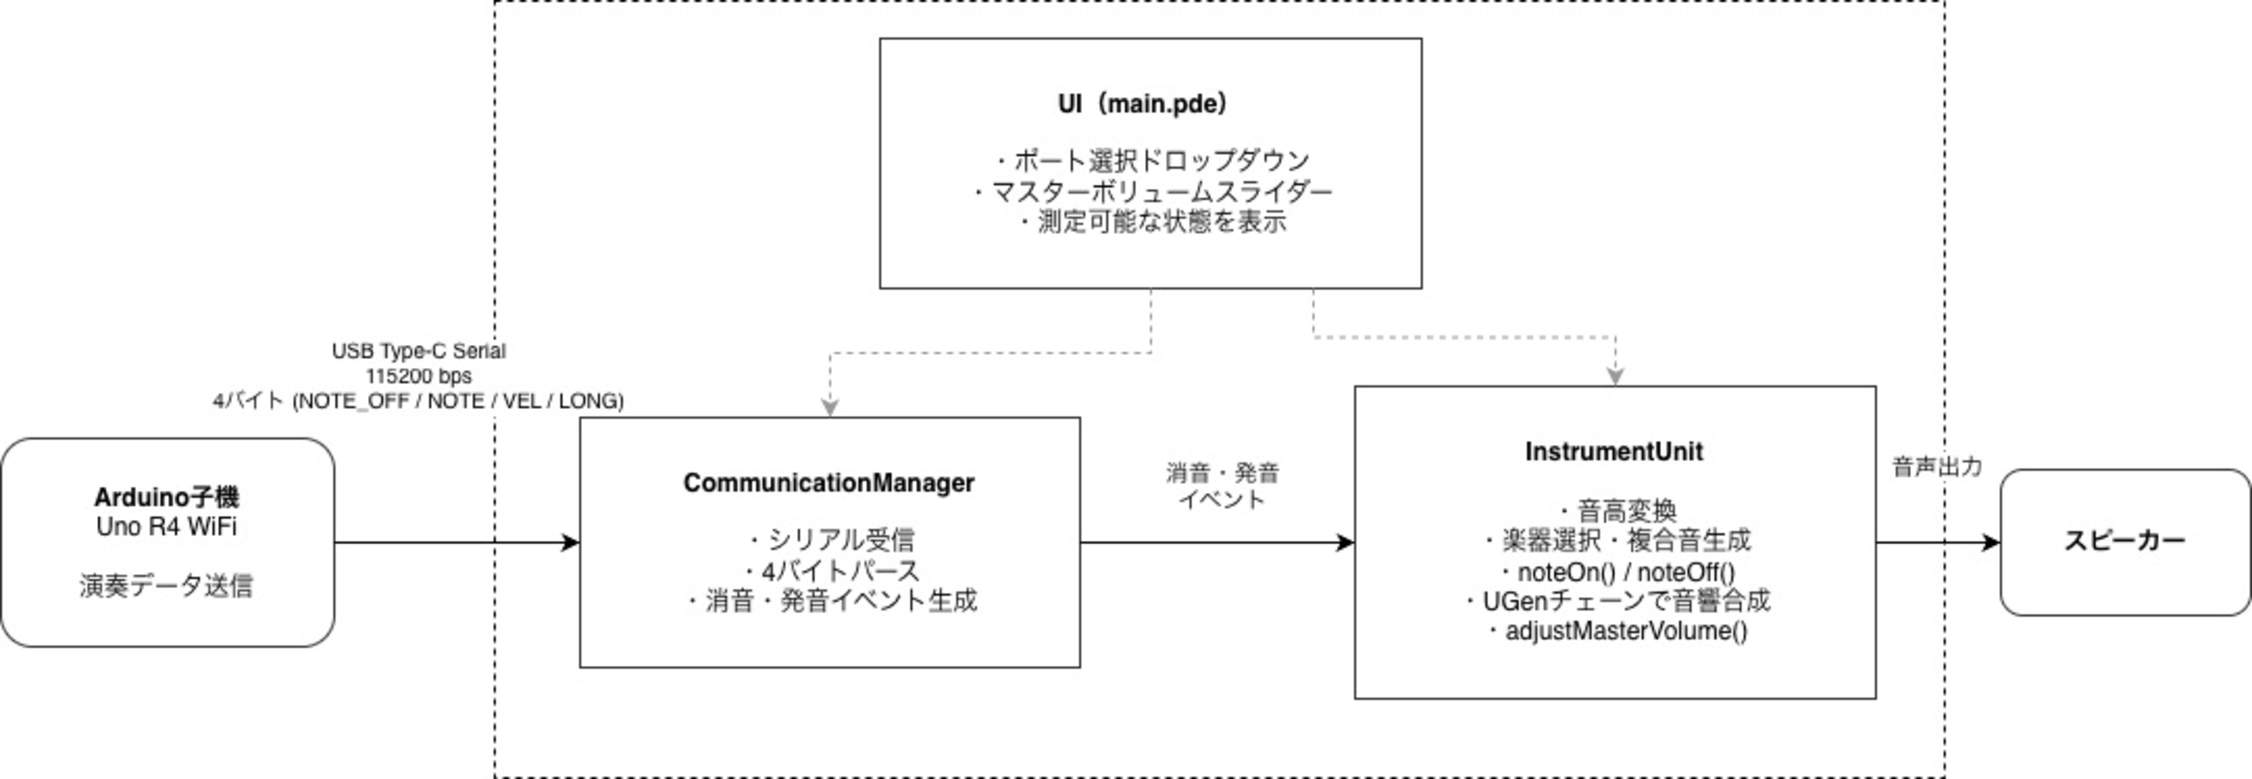
\includegraphics[width=0.8\linewidth]{figures/tantoD/system_diagram_D.pdf}
    \caption{担当Dシステム構成図}
    \label{fig:tantoD:system}
\end{figure}

図に示す通り，本システムは以下の3層で構成される．

\begin{description}
  \item[通信層 --- CommunicationManager]
  Arduino子機からUSB Type-C Serialを介して115200\,bpsで送信される
  4バイトパケット（NOTE\_OFF / NOTE / VEL / LONG）を受信・解析し，
  前音の消音および新規発音イベントとして音響層へ通知する．
  また，シリアルポートの自動接続およびログ出力を管理する．

  \item[音響合成層 --- InstrumentUnit]
  受信イベントに基づき，音高変換，楽器選択，波形生成，およびUGenチェーンによる
  音響合成処理を統括する．
  各楽器パートに対応するInstrumentUnitインスタンスを独立して保持し，
  多重発音にも対応する．

  \item[出力層 --- AudioOutput]
  Minimライブラリの\texttt{AudioOutput}を通じてスピーカーへ音響信号を送出する．
  マスターボリュームスライダーの値（0.0〜1.0）をデシベルに変換し，
  \texttt{out.setGain()}へ渡すことでアンサンブル全体の音量を調整可能とする．
\end{description}

各層間のデータフローを以下に示す．

\begin{center}
\texttt{Arduino子機} $\xrightarrow{\text{Serial 115200bps / 4B}}$
\texttt{CommunicationManager} $\xrightarrow{\text{発音・消音イベント}}$
\texttt{InstrumentUnit} $\xrightarrow{\text{UGenチェーン}}$
\texttt{AudioOutput} $\rightarrow$ \texttt{スピーカー}
\end{center}

なお，UGenチェーンの詳細（Oscil・ADSR・フィルタ・BitCrusherの接続構成）は
次節（音響合成チェーン）に示す．

\subsection{音響合成チェーン}
\label{sec:ugen}
受信したNOTE情報は，直ちに以下のUGenチェーンに渡され，
各楽器音がリアルタイムに合成・出力される．

\begin{center}
\texttt{Oscil（基音＋倍音）} $\rightarrow$
\texttt{ADSR} $\rightarrow$
\texttt{Filter（LowPassFS / HighPassFS）} $\rightarrow$
\texttt{BitCrusher} $\rightarrow$
\texttt{AudioOutput}
\end{center}

\begin{figure}[H]
    \centering
    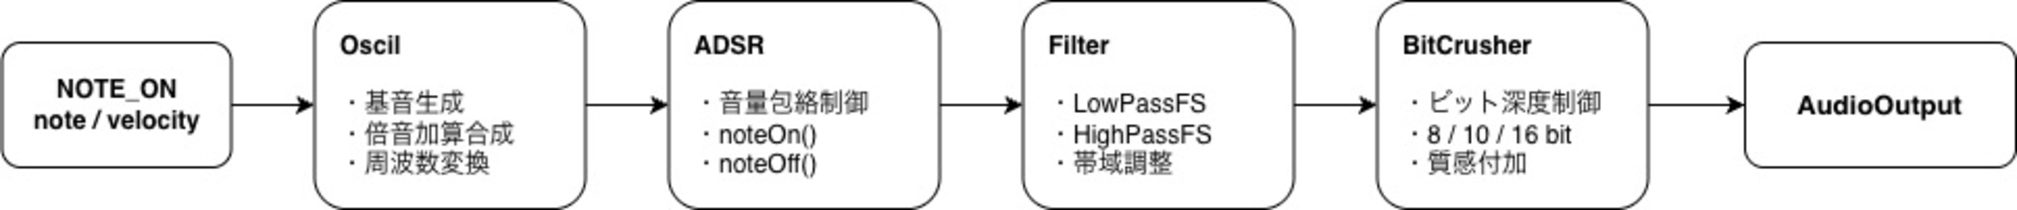
\includegraphics[width=0.8\linewidth]{figures/tantoD/ugen_chain_diagram.pdf}
    \caption{UGen合成チェーン図}
    \label{fig:tantoD:ugen}
\end{figure}

基音の生成から始まり，倍音の付加，ADSRによる音量エンベロープの適用，
フィルタによる帯域調整，BitCrusherによる質感付加を経て，
最終的なスピーカー出力となる．
各ユニットの詳細なパラメータ設定については詳細設計に示す．

なお本チェーンは有音程楽器（ピアノ・鉄琴・トランペット）およびバスドラムの標準形である．
実装上，ピアノはデジタル感を避けるためBitCrusherを省略し，
シンバルはOscilチェーンではなく事前生成したモーダル波形を\texttt{Sampler}経由で出力する．
また\texttt{HighPassFS}は現行実装では使用せず，全楽器\texttt{LowPass}である．

\subsection{操作インターフェース設計}
ハッカソン本番の現場における迅速なセットアップと，
開発・デバッグ時の動作確認を目的として，
Processing上に以下のコントロールパネルを実装する．

\subsubsection{シリアルポート接続（自動接続）}
各PCにおけるArduinoの認識状況（ポート名）が異なることを想定し，
起動時に\texttt{usbmodem}／\texttt{usbserial}を含むポートを自動的に探索して接続する．
該当がなければ先頭のポートに接続し，接続できない場合はキーボード入力による動作確認のみ可能とする．
接続状態（接続済み／未接続）は画面に表示し，現場での確認を支援する．

\subsubsection{マスターボリューム・コントロール}
5台のPCから出力される音量を合奏形式で調整するため，
0〜100\,\%の範囲で操作可能なマスターボリュームスライダーを設ける．
各PCのOS音量設定に依存することなく，
アンサンブルの聴感上のバランスをリハーサル中に即座に最適化できる．

\subsubsection{受信データモニタ}
開発・デバッグ時の動作確認を目的として，
受信した4バイトパケット（NOTE\_OFF / NOTE / VEL / LONG）の数値と，
シリアル接続状態（接続済み／未接続）をリアルタイムに表示するパネルを実装する．

設計当初はIDLE / PLAYING / FERMATA等のシステム状態表示を検討したが，
確定仕様の4バイトパケットには担当BのSTATE情報が含まれず，
Processing側で状態を確実に判定できないため，受信値そのもの（および接続状態）の表示とした．
なお，担当Cとの合意により4バイトパケットにSTATE情報（1バイト）を追加すれば，
状態表示へ拡張することが可能である．

\subsection{状態遷移図}
本システムはイベント駆動型であり，
Arduinoからのパケット受信をトリガとして動作する．
明示的な状態変数はもたず，発音中のボイス（\texttt{activeVoices}）の有無に応じて，
概念的にIDLE／PLAYINGの2状態として表せる．

\begin{figure}[H]
    \centering
    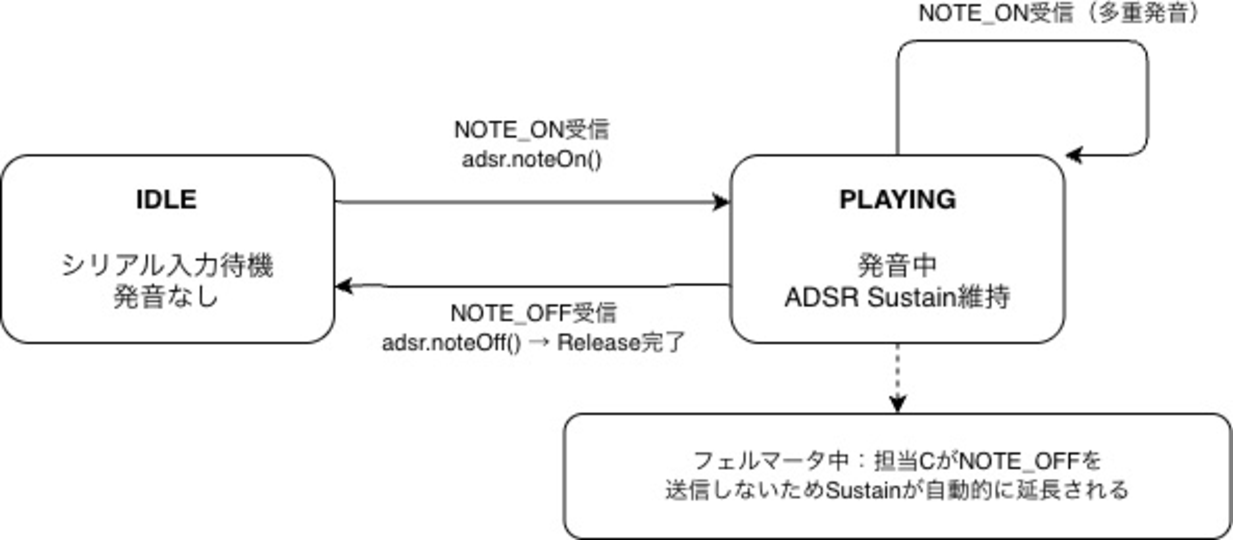
\includegraphics[width=0.8\linewidth]{figures/tantoD/state_transition_diagram_D.pdf}
    \caption{担当D状態遷移図}
    \label{fig:tantoD:state}
\end{figure}

\begin{description}
  \item[IDLE]
  発音中のボイスが存在しない状態（無音・入力待機）．
  発音パケット（NOTE $\neq$ 6）の受信により新規ボイスが生成され，PLAYINGへ移る．

  \item[PLAYING]
  1つ以上のボイスが発音中の状態．各ボイスはADSRに従って音を維持する．
  NOTE\_OFF=1を含む次パケットの受信で発音中のボイスがReleaseへ移行し，
  すべてのボイスが消えるとIDLEへ復帰する．
  フェルマータ中は担当Cが次パケットの送信を保留するため，Sustainが自動的に延長され，
  腕再開後に担当Cから次パケットが送信された時点でReleaseを開始する．
\end{description}

なお，各パートは専用スケッチとして1台のPCで独立に動作する（パート間は別プログラム）．
各パート内では1つのInstrumentUnitが複数のボイスを保持し，
各ボイスが独立したADSRライフサイクルをもつことで多重発音を実現する．